\documentclass[11pt]{article}

\usepackage[a4paper,margin=24mm]{geometry}
\usepackage{amsmath,amssymb}
\usepackage{array}
\usepackage{ragged2e}
\usepackage{booktabs}
\usepackage{graphicx}
\usepackage[numbers,sort&compress]{natbib}
\usepackage{xcolor}
\usepackage{placeins}
\usepackage{float}
\usepackage{hyperref}
\usepackage{microtype}
\setlength{\emergencystretch}{1.5em}

\hypersetup{
  colorlinks=true,
  linkcolor=blue!55!black,
  citecolor=blue!55!black,
  urlcolor=blue!55!black,
  pdftitle={Conservative Euler--BIE/VOF coupling for overturning free-surface waves over variable bathymetry},
  pdfauthor={Saveliy Baturin}
}
\graphicspath{{../research/results/publication_package/}{../research/results/q_transport/}}
\newcommand{\dd}{\,\mathrm{d}}

\title{Conservative Euler--BIE/VOF coupling for overturning free-surface waves over variable bathymetry}
\author{Saveliy Baturin}
\date{}

\begin{document}
\maketitle

\begin{abstract}
A hybrid method is developed for two-dimensional overturning waves over
variable bathymetry.  A fully nonlinear Euler boundary-integral equation
(BIE) advances the irrotational pre-contact flow, while an embedded two-phase
volume-of-fluid (VOF) solver provides the continuation when the interface
approaches self-contact.  The BIE combines Kress product quadrature with a
nonlocal-gap trigger for oversampled close evaluation and represents the
adaptive boundary state by integrated panel circulations.  At transfer, shared
face-averaged BIE fluxes are projected onto a vertex streamfunction; the
resulting MAC face field is divergence-free by construction.  The liquid
aperture $q=f c_s$ is then transported with a shared embedded-boundary flux,
including an exact pure-state rule and a capacity restriction confined to the
mixed-interface band.

Verification separates operator accuracy, conservation and interface
geometry.  On a manufactured folded boundary, oversampling reduces the
relative Dirichlet-to-Neumann error from 6.36 to $6.91\times10^{-2}$ at 64
panels despite similarly small linear residuals.  A solitary-wave translation
has shape and speed errors $1.82\times10^{-5}$ and
$8.40\times10^{-5}$.  Manufactured aperture transport is first-order on the
three finest grids and preserves liquid volume and $0\le q\le c_s$ to
roundoff.  The constrained handoff has 1.68\% face-flux error, 3.12\% surface
velocity error and $1.07\times10^{-14}$ face-divergence RMS.

The coupled breaker is continued to nondimensional time 6 on three nested
receiver grids.  Maximum relative liquid-volume drift is
$8.56\times10^{-8}$, $6.43\times10^{-8}$ and $5.67\times10^{-9}$ on levels
8--10, with no aperture-bound violation.  Level 10 produces a transient
disconnected gas component at $t=1.96$, but the event is absent at the two
coarser levels and its detected onset varies by 0.06 under conservative raster
coarsening.  At $t=6$, the level-9/10 upper-profile and crest differences are
8.18\% and 6.25\%.  The method therefore achieves stable conservative
continuation and exposes a resolution-dependent topology transition, but the
present calculation does not establish grid-converged wave impact or air
entrainment.
\end{abstract}

\section{Introduction}

Boundary-integral descriptions of inviscid water waves resolve vertical and
overturning free surfaces without a height-function restriction
\cite{LonguetHigginsCokelet1976,DoldPeregrine1986,BakerMeironOrszag1982}.
They remain efficient while the liquid is irrotational and the interface is a
single non-self-intersecting curve, but cease to describe entrained air,
vorticity production and topology change after impact.  Fully nonlinear BEM
calculations have reproduced solitary-wave shoaling and classified breaking
regimes over beaches and obstacles \cite{GrilliSvendsenSubramanya1997}, while
two-phase VOF methods naturally continue through interface reconnection.

Hybridisation alone is not new.  Khait and Ma coupled a quasi-potential BEM to
a two-phase incompressible VOF solver for breaking wave trains
\cite{KhaitMa2021}.  Kanehira et al. recently embedded a GPU-SPH region in a
three-dimensional fully nonlinear potential-flow calculation and compared jet
and cavity dynamics with experiments \cite{KanehiraEtAl2026}.  The numerical
question considered here is narrower: can an adaptive circulation-carrying
BIE state be transferred to an embedded two-phase receiver while conserving
the appropriate liquid measure and satisfying the receiver's discrete
divergence and momentum constraints?

The method has four coupled elements.  First, a nonlocal geometric indicator
activates oversampled quadrature when two parameter-distant surface branches
approach.  Second, integrated panel circulation is preserved under adaptive
redistribution.  Third, face-averaged velocity rather than independent
cell-centred samples is transferred to a divergence-conforming MAC field.
Fourth, the full-cell liquid aperture $q=f c_s$ is transported by a shared
VOF/embedded-boundary flux.  The calculations below test these components and
then apply the complete coupling to an overturning breaker on three receiver
grids.

\section{Mathematical formulation}

\subsection{Pre-contact free-surface flow}

Let $\Omega(t)\subset\mathbb{R}^2$ be the liquid domain.  With velocity
$\boldsymbol u=\nabla\phi$, the potential satisfies
\begin{equation}
 \nabla^2\phi=0\quad\text{in }\Omega(t),\qquad
 \partial_n\phi=0\quad\text{on the bed }\Gamma_b.
 \label{eq:laplace}
\end{equation}
The periodic free surface is
$\boldsymbol X(\alpha,t)=(x(\alpha,t),z(\alpha,t))$ and carries the trace
$\psi=\phi|_{\Gamma_f}$.  With normal velocity $V_n=\partial_n\phi$,
tangential fluid velocity $V_t=\partial_s\psi$ and freely chosen marker
velocity $W_t$, the surface equations are
\begin{align}
 \boldsymbol X_t &= V_n\boldsymbol n+W_t\boldsymbol t,\\
 \psi_t &= \tfrac12V_n^2-\tfrac12V_t^2+W_tV_t-gz.
 \label{eq:surface-evolution}
\end{align}

For prescribed $\psi_f$ and zero bed flux, Green's identity gives the mixed
system
\begin{equation}
\begin{bmatrix}S_{:f}&-(\tfrac12I+K)_{:b}\end{bmatrix}
\begin{bmatrix}q_f\\ \phi_b\end{bmatrix}
=(\tfrac12I+K)_{:f}\psi_f,
\label{eq:mixed-bie}
\end{equation}
where $q_f=\partial_n\phi|_{\Gamma_f}$ and $S$ and $K$ are the periodic
single- and double-layer operators.  Their Green function is
\begin{equation}
G_L(\Delta x,\Delta z)=-\frac{1}{4\pi}\log\!\left[
2\left(\cosh\frac{2\pi\Delta z}{L}-
\cos\frac{2\pi\Delta x}{L}\right)\right].
\end{equation}
Kress product weights integrate the logarithmic self interaction.  The
incident-wave normal velocity is projected onto the actual bathymetry by
subtracting its mean boundary flux and solving the compatible Neumann problem
in a zero-mean gauge.

The ordinary self rule becomes under-resolved when two distant arclength
segments approach.  Define
\begin{equation}
d_{\rm nl}=\min_{d_s(i,j)>8\overline{\Delta s}}
\|\boldsymbol X_i-\boldsymbol X_j\|,
\qquad
\overline{\Delta s}=\frac{2\pi}{N}\overline{|\boldsymbol X_\alpha|}.
\end{equation}
When $d_{\rm nl}/\overline{\Delta s}<1.5$, the complete free-surface
self block is reevaluated after trigonometric interpolation to $pN$ points,
with
\begin{equation}
p=\operatorname{clip}_{[2,16]}
\left\lceil4\overline{\Delta s}/d_{\rm nl}\right\rceil.
\end{equation}
The density and geometry are oversampled together so that the Kress splitting
remains consistent.

\subsection{Adaptive circulation representation}

The surface potential trace is equivalently represented by sheet strength
$\gamma=-\partial_s\psi$.  For a panel $j$ the integrated circulation
\begin{equation}
 \Gamma_j=-\int_{s_j}^{s_{j+1}}\gamma\,\dd s
          =\psi_{j+1}-\psi_j
 \label{eq:panel-circulation}
\end{equation}
is used as the conservative carrier during marker redistribution.  New panel
endpoints are chosen from a smoothed monitor depending on curvature, sheet
strength and inverse nonlocal gap; the cumulative circulation is interpolated
monotonically and then differenced on the new partition.  This preserves total
circulation to roundoff.  These boundary circulations represent the
irrotational potential trace; they are not bulk material vortices.

\subsection{Conservative embedded liquid aperture}

For a Cartesian receiver cell $K_i$, define the full-cell physical liquid
aperture
\begin{equation}
q_i=\frac{|K_i\cap\Omega_\ell\cap\Omega_f|}{|K_i|},
\qquad 0\le q_i\le c_{s,i},
\label{eq:q-definition}
\end{equation}
where $c_s$ is the open-fluid volume fraction and $f=q/c_s$ is conditional on
the open part of the cell.  This full-cell measure is consistent with
solid-aware VOF/embedded-boundary formulations and conservative contact-line
treatments \cite{TavaresEtAl2024,ChenEtAl2025,HuangEtAl2025,HuangEtAl2026}.
One oriented swept volume is assigned to every
shared face,
\begin{equation}
F_e=|S_e(\Delta t)\cap\Omega_\ell\cap\Omega_f|,
\qquad
q_i^{n+1}=q_i^n-|K_i|^{-1}
\sum_{e\subset\partial K_i}\operatorname{sgn}(i,e)F_e.
\label{eq:q-flux}
\end{equation}
Because the same $F_e$ enters adjacent cells with opposite signs, global
liquid volume telescopes exactly.  A pure donor satisfies
$F_{\ell,e}=0$ for $f_d=0$ and $F_{\ell,e}=F_{f,e}$ for $f_d=1$; only genuinely
mixed cut cells require a capacity restriction.  The restriction is applied
to mixed cells and their face-connected one-cell halo,
\begin{equation}
\Delta t\le0.45\min_{i\in\mathcal I}
\frac{c_{s,i}\Delta_i}
{\max_{e\subset\partial K_i}|u_e f_{s,e}|}.
\label{eq:cut-cell-step}
\end{equation}

\subsection{Divergence-conforming state transfer}

The target liquid momentum is evaluated from boundary data,
\begin{equation}
\boldsymbol P^\star=\rho\int_\Omega\nabla\phi\,\dd A
=\rho\oint_{\partial\Omega}\phi\boldsymbol n\,\dd s.
\label{eq:target-momentum}
\end{equation}
Two-point Gauss quadrature supplies the BIE velocity averaged over every
receiver face.  A periodic vertex streamfunction $\chi$ then defines
\begin{equation}
u_{i-1/2,k}=\frac{\chi_{i-1/2,k+1/2}-\chi_{i-1/2,k-1/2}}{\Delta z},
\quad
w_{i,k-1/2}=-\frac{\chi_{i+1/2,k-1/2}-\chi_{i-1/2,k-1/2}}{\Delta x}.
\label{eq:mac-curl}
\end{equation}
The standard face-difference divergence of this field vanishes identically.
Compatibility projections and divergence-preserving transfer between
non-conforming or multilevel grids provide the relevant numerical context
\cite{SunWheeler2006,CervoneManservisiScardovelli2011,GorgesEtAl2022}.
The sparse fit minimises
\begin{equation}
\|W_f(C_h\chi-\bar{\boldsymbol u})\|_2^2
+\lambda_s\|S\chi-\boldsymbol u_s\|_2^2
+\lambda_b\|B\chi\|_2^2
+\lambda_P\|M\chi-\boldsymbol P^\star/\rho\|_2^2
+\lambda_e\|E\chi\|_2^2+\lambda_h\|L_h\chi\|_2^2.
\label{eq:mac-fit}
\end{equation}
Here $B\chi=0$ makes the bed a streamline, $M$ imposes momentum, $E$ suppresses
exterior kinetic energy and $L_h$ regularises unconstrained modes.  After AMR,
the face flux transported by the mesh is retained and a receiver-grid
Helmholtz correction restores compatibility; no global velocity shift is
applied.

\section{Verification}

The tests are grouped by the property they measure.  Analytic and manufactured
solutions test the BIE and aperture operators; algebraic residuals test the
handoff constraints; long coupled runs test conservation and boundedness.
Interface contact is assessed separately in Section~\ref{sec:breaker}.

For a flat surface Fourier mode, the Dirichlet-to-Neumann eigenvalue and the
discrete velocity agree to machine precision.  A fully nonlinear solitary
wave propagated over one reference interval has relative shape error
$1.82\times10^{-5}$ and speed error $8.40\times10^{-5}$.  On a manufactured
folded interface, the unoversampled 64-panel discretisation has a relative DNO
error of 6.36 even though its linear residual is near $10^{-13}$; order-16
oversampling reduces the error to $6.91\times10^{-2}$
(figure~\ref{fig:close-quadrature}).

\begin{figure}[t]
\centering
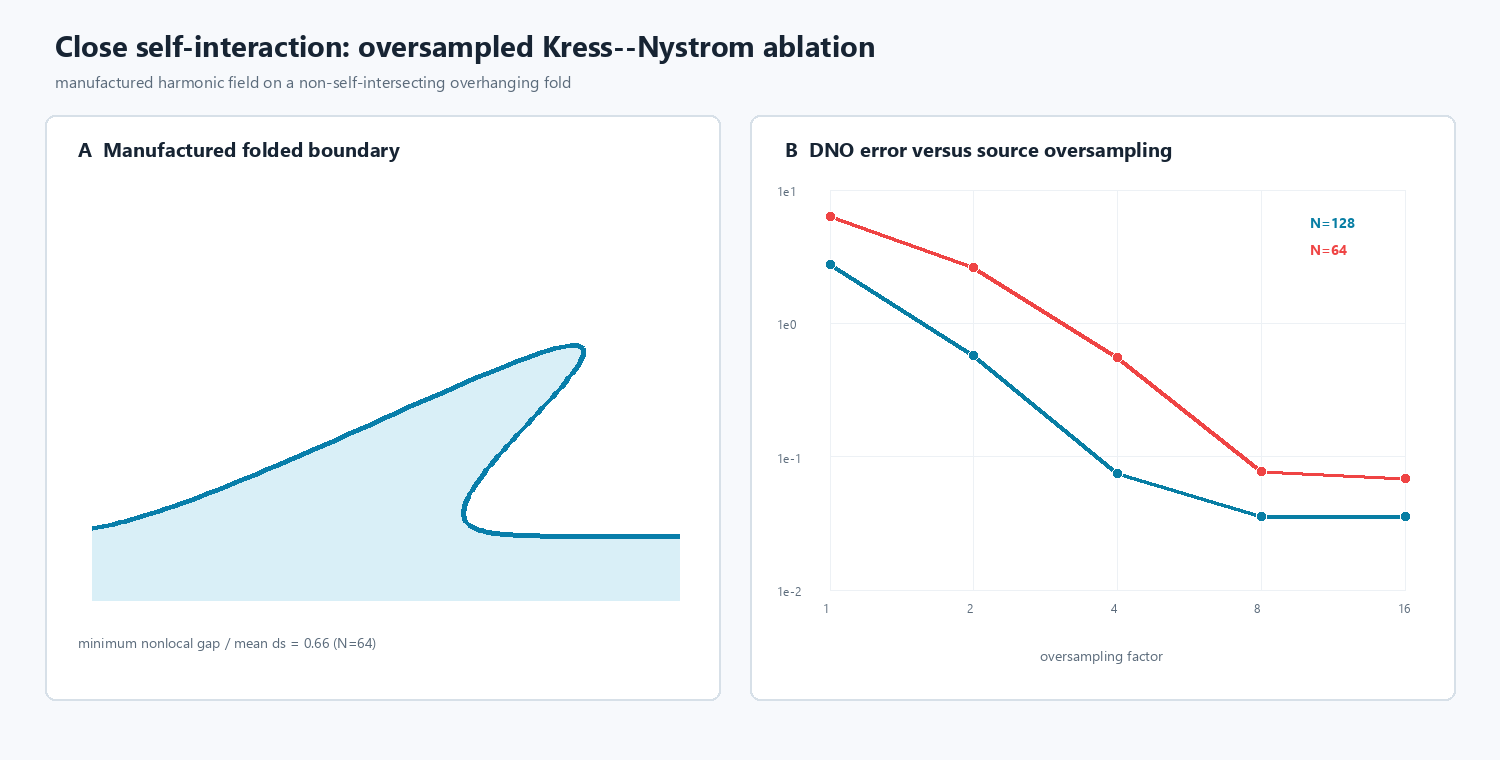
\includegraphics[width=0.88\linewidth]{near_self_quadrature_ablation.png}
\caption{Close-interaction quadrature on a manufactured folded interface.
The boundary-integral residual alone does not diagnose the unresolved
parameter-distant branch; geometric oversampling reduces the DNO error.}
\label{fig:close-quadrature}
\end{figure}

For sinusoidal-interface translation, the relative $L^1(q)$ errors on levels
6--8 are 0.01378, 0.007689 and 0.003538, corresponding to observed orders 0.84
and 1.12.  Fixed, frozen-AMR and every-step-AMR volume drift remains below
$2.0\times10^{-13}$.  An inclined-wall test gives errors 0.02325, 0.01247 and
0.006154 on levels 7--9 (orders 0.90 and 1.02) while preserving volume and
bounds to roundoff.  Restricting the cut-cell timestep to the interface band
requires 211 steps at level 7, compared with 758 when every cut cell is
included.

Independent cell-centred samples of the late BIE velocity have a 15.92\%
best-fit error in the range of the receiver curl.  Shared face averages followed
by equation~\eqref{eq:mac-fit} reduce the face-flux error to 1.6835\% and the
surface-velocity error to 3.1229\%.  Relative momentum error is
$1.99\times10^{-9}$ and the finite-volume divergence RMS is
$1.07\times10^{-14}$.  GPU sparse LSQR takes 12.76~s versus 69.54~s for the CPU
solve and changes the trusted-face field by only $4.58\times10^{-8}$ relative
(figure~\ref{fig:handoff}).  This acceleration applies to the sparse handoff
fit; the two-phase evolution reported below is CPU-serial.

\begin{figure}[t]
\centering
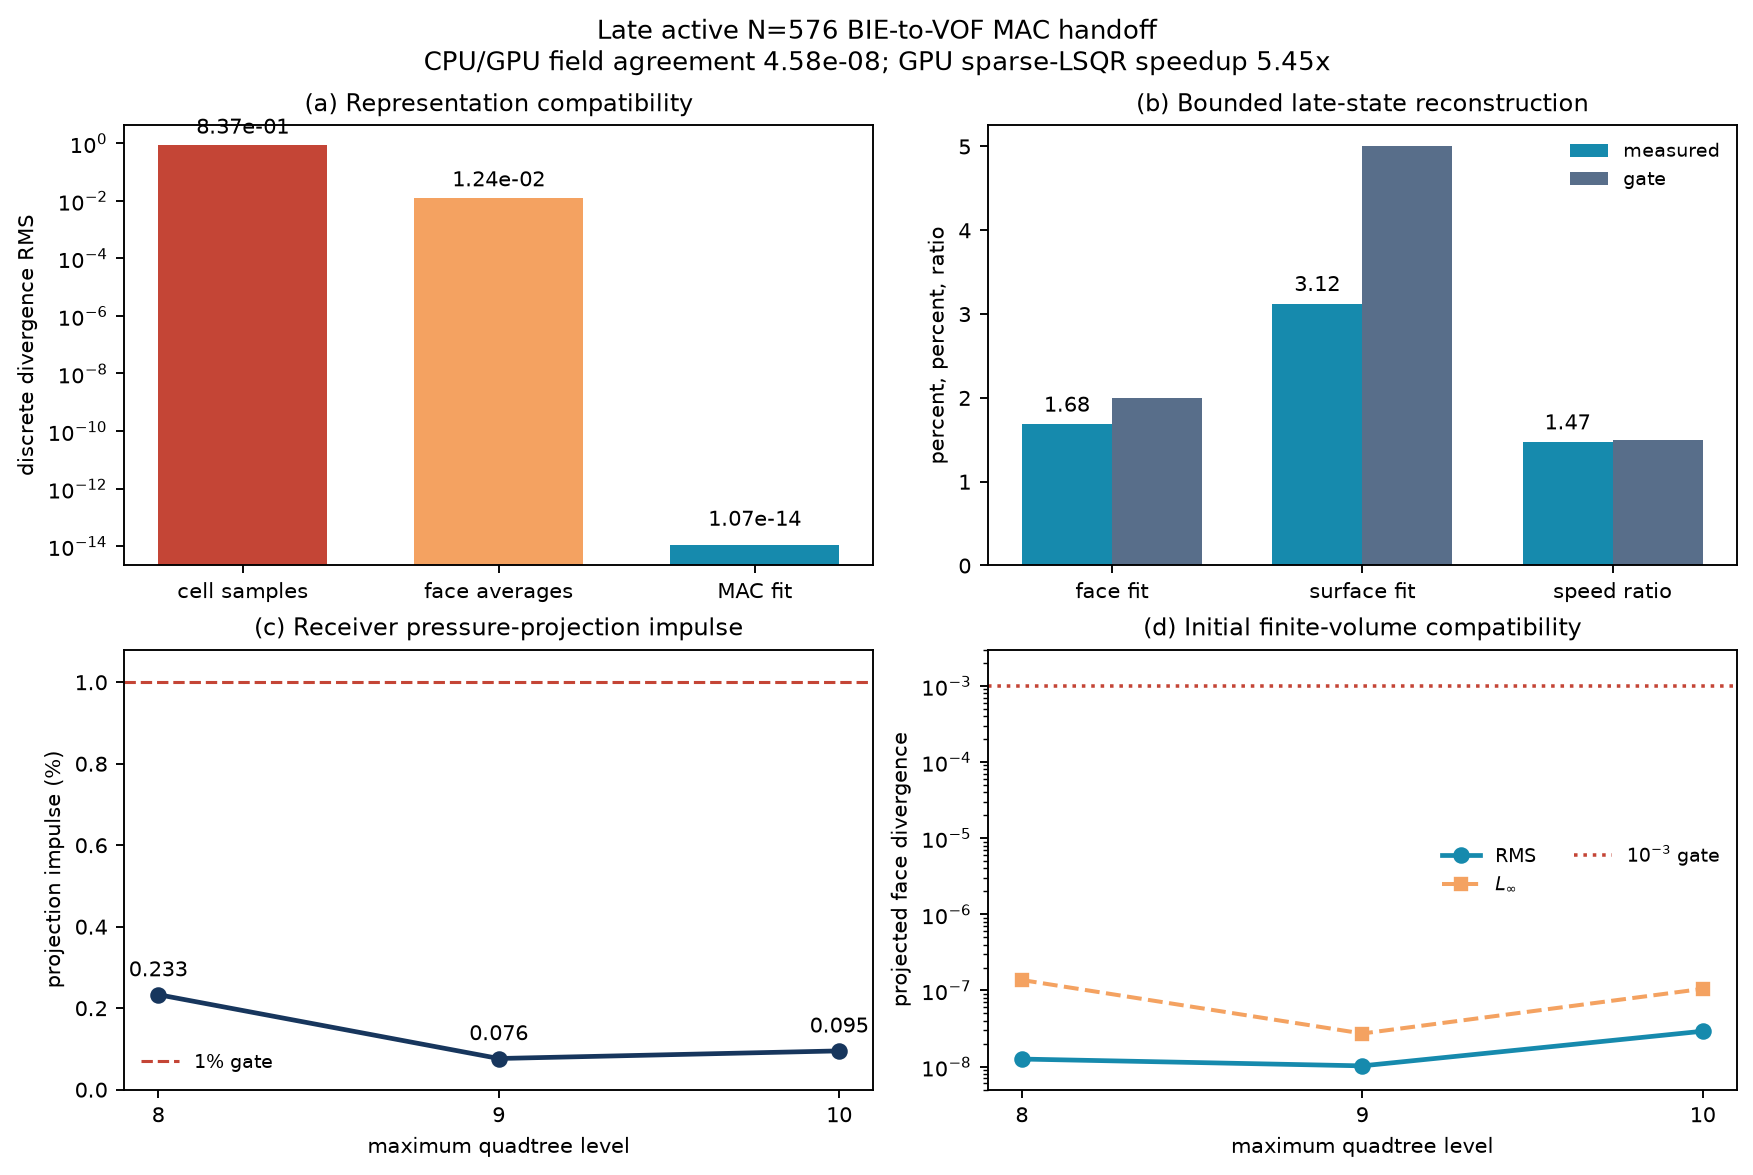
\includegraphics[width=0.96\linewidth]{mac_face_handoff_audit.png}
\caption{Compatible transfer of the late BIE state.  Face averaging reduces
the initial representation mismatch and the streamfunction curl enforces
finite-volume divergence compatibility.  Receiver mass, momentum and
post-projection divergence are shown for levels 8--10.}
\label{fig:handoff}
\end{figure}

\section{Three-grid overturning-wave experiment}
\label{sec:breaker}

\subsection{Configuration and event definition}

The source is an active $N=576$ BIE state over a periodic $1{:}30$ beach and
return slope, transferred at nondimensional BIE time 20.303125.  Conservative
raster overlap changes volume by $2.45\times10^{-13}$ relative to the source;
reconciliation with the analytic embedded bed changes 0.0868\%.  Receiver
maximum levels 8, 9 and 10 use minimum levels 6, 7 and 8, respectively, and
adapt after every accepted physical step.  VOF and vorticity fields are sampled
every 0.02 through continuation time 6.

A gas component is classified as a resolved closure if it is disconnected
from the exterior, does not touch a one-finest-cell bed guard, has area at least
$\Delta^2$, and persists for three output frames.  Four-neighbour components
are joined across the horizontal periodic seam.  Diagnostic coarsening uses
exact block liquid-area fractions at scale factors two and three and thresholds
0.25, 0.5 and 0.75.  The accepted onset-time variation is at most 0.04.

\subsection{Conservation and topology}

All three continuations remain bounded to $t=6$.  Table~\ref{tab:three-grid}
summarises the invariant and compatibility histories.  The aperture bounds
hold to roundoff.  The largest post-AMR divergence and relative momentum and
kinetic-energy corrections remain below $3.86\times10^{-9}$,
$8.24\times10^{-5}$ and $9.31\times10^{-6}$, respectively.

\begin{table}[t]
\centering
\small
\caption{Three-grid coupled continuation through $t=6$.  $A_{\max}$ is the
largest exterior-disconnected, bed-detached gas area before the one-cell area
filter.}
\label{tab:three-grid}
\begin{tabular}{rrrrrr}
\toprule
Level & $\max|\delta V/V|$ & $\max|D_h\boldsymbol u|_\infty$ &
$\max|\delta P/P|$ & $A_{\max}/\Delta^2$ & resolved onset \\
\midrule
8  & $8.56\times10^{-8}$ & $3.59\times10^{-10}$ & $8.24\times10^{-5}$ & 0     & none \\
9  & $6.43\times10^{-8}$ & $2.32\times10^{-10}$ & $4.04\times10^{-5}$ & 0.498 & none \\
10 & $5.67\times10^{-9}$ & $3.86\times10^{-9}$  & $6.40\times10^{-5}$ & 10.57 & 1.96 \\
\bottomrule
\end{tabular}
\end{table}

Level 8 has no disconnected gas component.  Level 9 develops a late component
whose maximum area is only $0.498\Delta_9^2$.  Level 10 develops a component
larger than ten finest-cell areas near $t=1.96$, but it has disappeared by
$t=2.08$.  Across the seven conservative raster probes its onset ranges from
1.90 to 1.96, exceeding the 0.04 tolerance.  A later group of cavities at
$t=5.10$ is likewise absent on the coarser grids.  Thus the algebraic
conservation properties converge more strongly than the observed topology
(figures~\ref{fig:three-grid-invariants} and \ref{fig:same-time}).

\begin{figure}[t]
\centering
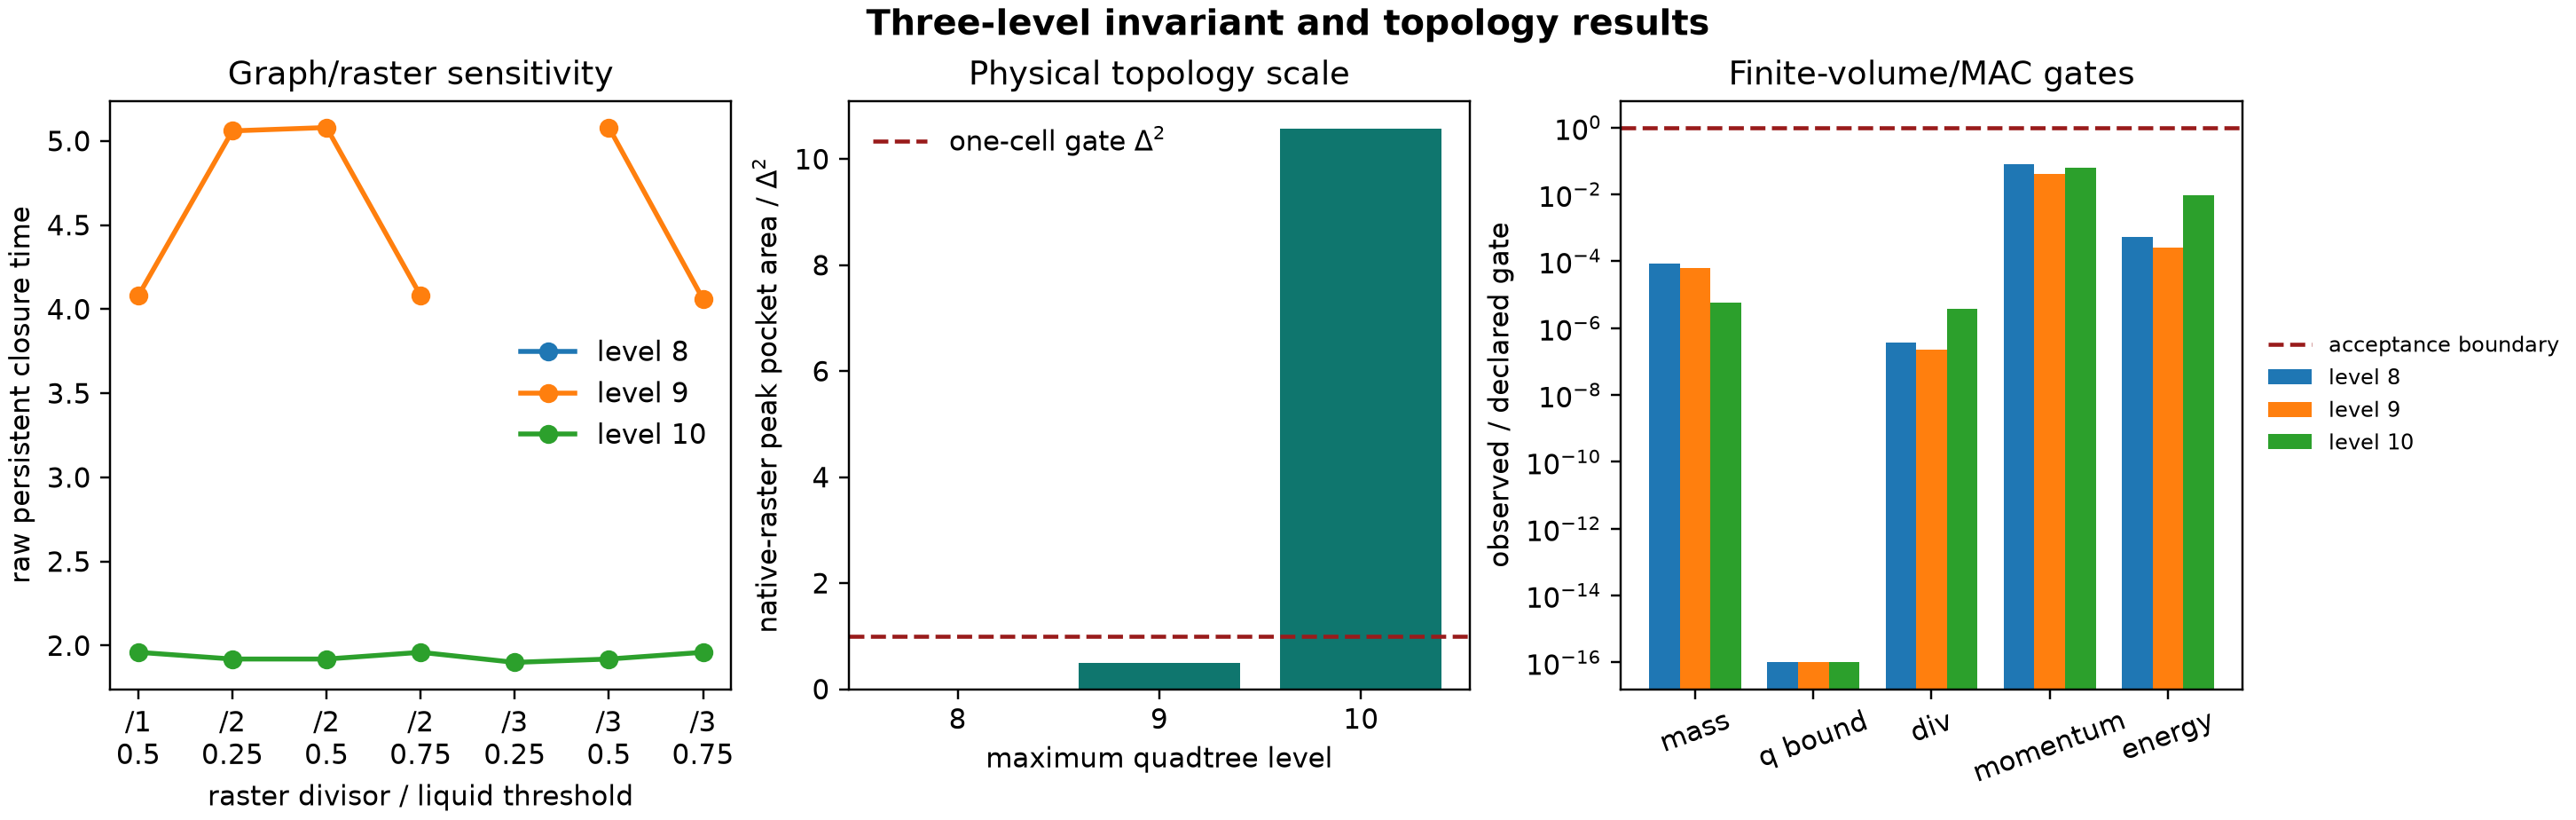
\includegraphics[width=\linewidth]{impact_claim_q_l8_l9_l10_audit.png}
\caption{Raster sensitivity, gas-component scale and normalized conservation
and MAC compatibility measures.  The level-10 component is physically larger
than one finest cell, but its time and existence are not reproduced across
the receiver grids.}
\label{fig:three-grid-invariants}
\end{figure}

\begin{figure}[H]
\centering
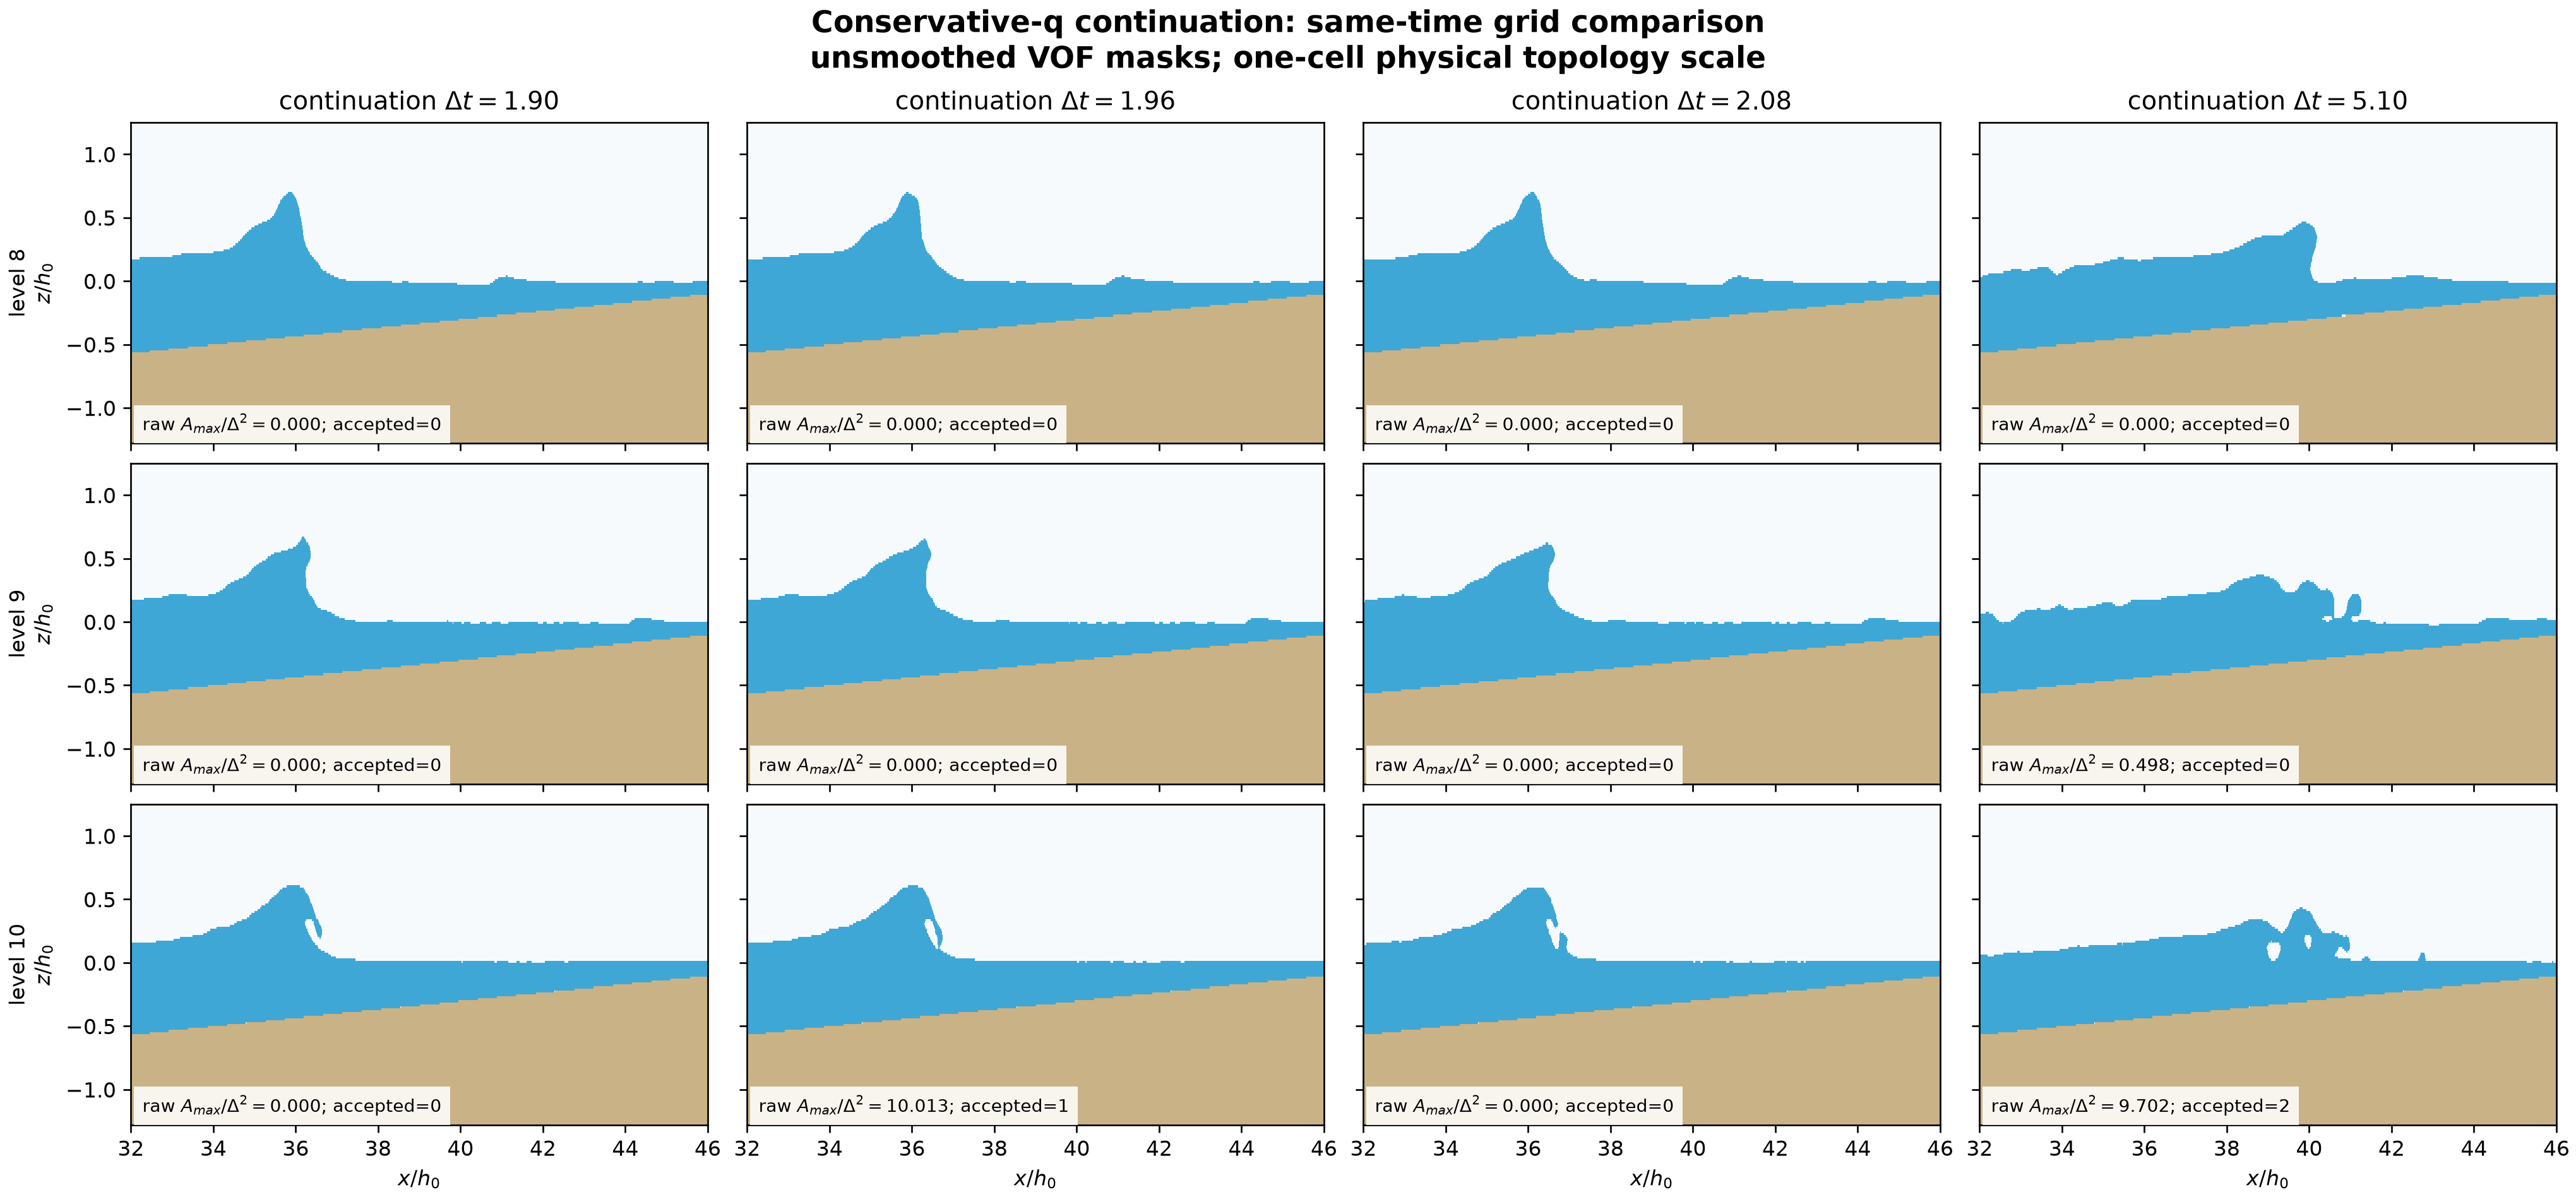
\includegraphics[width=\linewidth]{impact_claim_q_l8_l9_l10_grid_comparison.png}
\caption{Unsmoothed VOF masks at matched continuation times.  The transient
level-10 cavity at $t=1.96$ and the later cavities at $t=5.10$ are not
same-time features of levels 8 and 9.  Labels report the largest raw component
in units of the local finest-cell area and the number passing the physical
area filter.}
\label{fig:same-time}
\end{figure}

\subsection{Geometric refinement}

Upper-surface profiles are extracted at identical physical times without
interpolation between frames.  Relative RMS differences are normalised by the
initial level-10 amplitude.  The maximum L8/L9 and L9/L10 profile differences
over $0\le t\le6$ are 11.39\% and 8.26\%; at $t=6$ they are 8.12\% and 8.18\%.
The final L9/L10 crest difference is 6.25\%, with a maximum of 12.5\%.
Although the instantaneous Richardson indicator is positive for 80.4\% of the
last time unit, the fine-pair profile and crest differences both exceed the
5\% tolerance (figure~\ref{fig:three-grid-geometry}).

\begin{figure}[H]
\centering
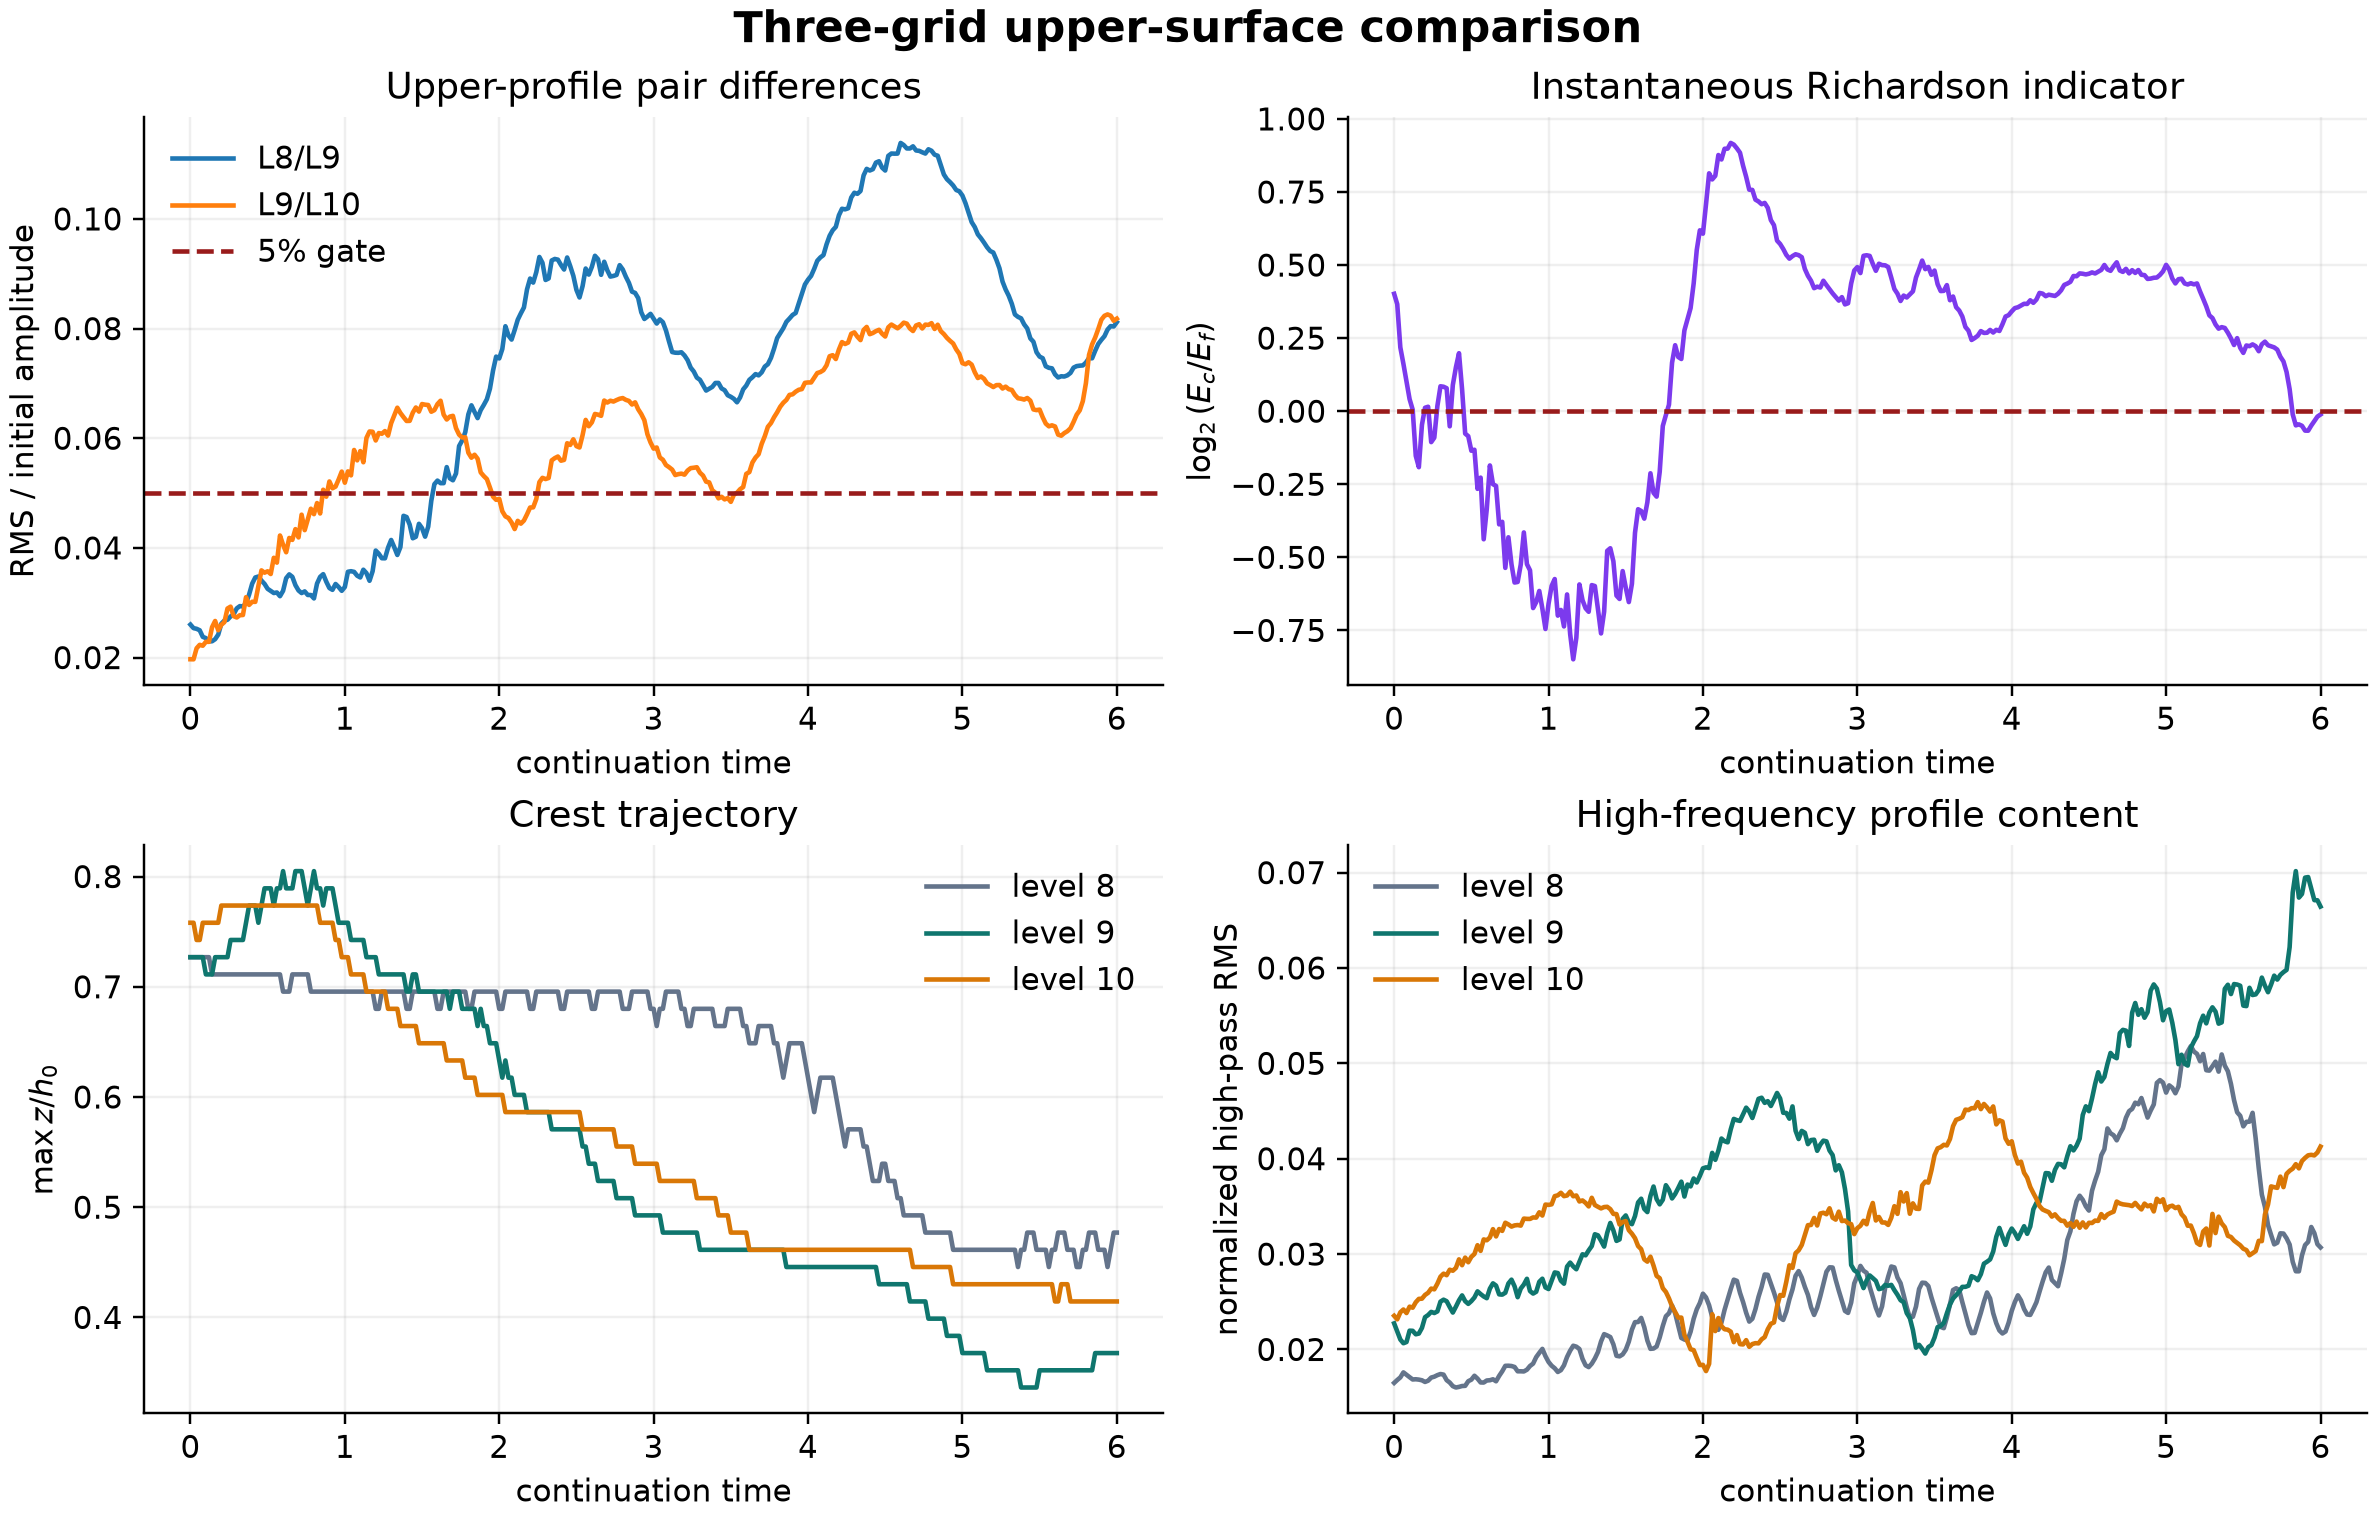
\includegraphics[width=0.98\linewidth]{impact_claim_q_l8_l9_l10_morphology.png}
\caption{Three-grid upper-surface comparison.  Pairwise profile errors remain
above the 5\% tolerance for much of the continuation, and the final fine-pair
profile and crest differences are 8.18\% and 6.25\%.}
\label{fig:three-grid-geometry}
\end{figure}

The mismatch is not captured by smooth-profile measures alone.  On level 9,
adapting every second or fourth step changes the upper-profile RMS by at most
3.55\% but shifts the first raw subcell component from $t=4.08$ to about 5.1.
Topology is therefore more sensitive to mesh evolution than the bulk profile.

The level-10 vorticity field contains a concentrated signed layer around the
curling crest and beneath the emerging cavities
(figure~\ref{fig:vorticity}), consistent with the localisation reported in
small-viscosity plunging-wave calculations \cite{RiquierDormy2024}.  The plotted markers sample the Eulerian
vorticity quadrature $\Gamma_{ij}\simeq\omega_{ij}\Delta A$; they are not
Lagrangian particles.  Quantitative post-contact circulation requires a
separate refinement study because potential-flow sheet labels cannot be
continued through reconnection.

\begin{figure}[H]
\centering
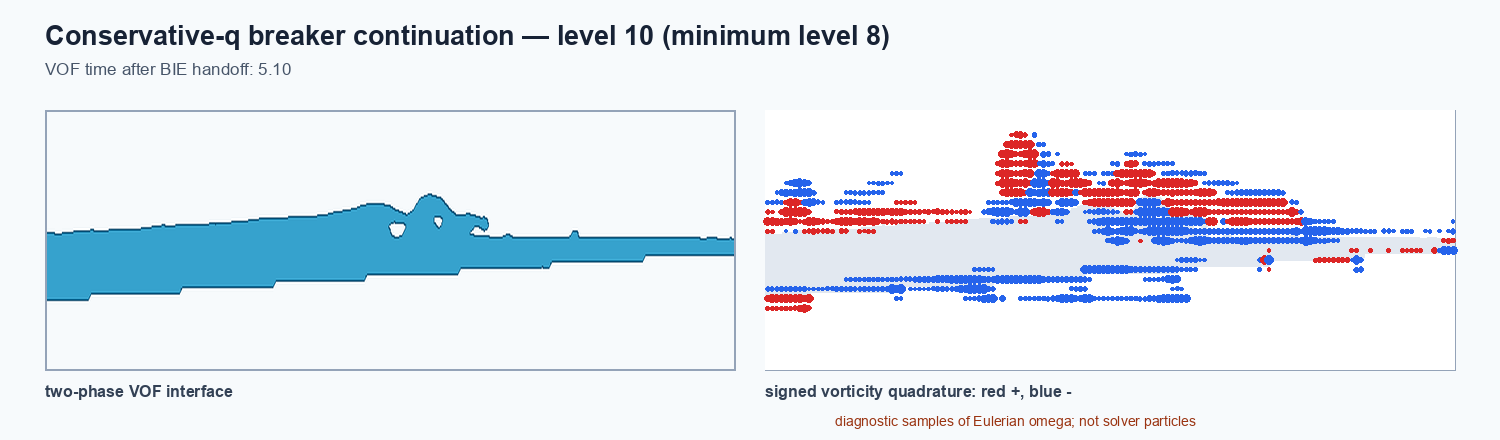
\includegraphics[width=\linewidth]{impact_claim_q_l10_vorticity_points_keyframes/late_pocket.png}
\caption{Level-10 state at $t=5.10$.  Left: two-phase VOF interface.  Right:
signed samples of the resolved Eulerian vorticity (red positive, blue
negative).}
\label{fig:vorticity}
\end{figure}

\section{Discussion}

The experiment separates stability from physical convergence.  Transporting
$q$ with shared embedded fluxes removes the previous long-time mass loss, and
the receiver-grid correction retains divergence and momentum compatibility
after AMR.  These properties remain stable through 301 output times on all
three grids.  They do not, however, determine the topology of the free
surface: the first resolved gas component appears only on level 10 and is
transient, while the upper-surface geometry remains outside the selected
fine-grid tolerance.

The level-10 cavity may be the first resolved representation of jet closure,
or it may be a resolution-dependent branch selected by the coupled AMR and
interface reconstruction.  The current data cannot distinguish these
possibilities.  A decisive impact calculation requires at least one finer
receiver grid, time-step refinement, several earlier handoff times and an
aligned experimental or high-resolution two-phase reference.  Event time,
jet-tip position, enclosed-gas area and pressure impulse should converge
together.  Air compressibility and three-dimensionality may also become
important near closure.

The contribution is therefore the conservative and divergence-conforming
coupling, together with a three-level observation that topology converges more
slowly than invariants.  A matched end-to-end accuracy--cost comparison with a
contemporary BEM--VOF or potential-flow/particle hybrid remains necessary to
establish an efficiency advantage.  The present GPU timing concerns only the
sparse handoff reconstruction; the serial two-phase solve dominates the
reported continuation cost.

\section{Conclusions}

An adaptive Euler--BIE state can be transferred to an embedded two-phase VOF
receiver without sacrificing the receiver's discrete divergence structure.
The essential choices are to transfer shared face averages, construct the MAC
field as a streamfunction curl, impose momentum in the receiver quadrature and
transport the full-cell liquid aperture $q=f c_s$ with a shared
embedded-boundary flux.

Manufactured tests show first-order aperture convergence with roundoff mass
and bound preservation.  The coupled L8--L10 breaker remains bounded through
$t=6$, with maximum relative liquid-volume drift below
$8.57\times10^{-8}$ and small post-AMR compatibility corrections.  The
level-10 trajectory contains a resolved but transient gas component and
strong crest vorticity.  Its onset and morphology are not reproduced on the
coarser grids, and the final L9/L10 profile and crest differences exceed 5\%.

The present result supports a conservative hybrid continuation method and
identifies a resolution-dependent topology transition.  It does not yet
support a grid-converged prediction of plunging impact, trapped-air volume or
impact impulse.

\section*{Data and code availability}

Source code, solver inputs, machine-readable diagnostics and scripts used to
produce the figures are available in the accompanying research repository.
The BIE input data and external comparison data retain their original
licences.  The two-phase calculations use a pinned Basilisk environment; the
exact revision and compile parameters are supplied with the archived runs.

\bibliographystyle{plainnat}
\bibliography{references}

\end{document}
